% -*- coding: utf-8 -*-

\begin{chapter}{Уравнение движения}\label{chap:7}
% \chapter[The Equations of Motion]{Some Mathematics: The Equations of Motion}
В этой главе мы рассмотрим, как жидкость реагирует на приложенные к ней 
внешние и внутренние силы. Это приведёт нас к выводу некоторых основных 
уравнений, описывающих динамику океана. В следующей главе мы обсудим влияние 
вязкости, а в главе~\ref{chap:12}~--- последствия завихренности.
%
% In this chapter I consider the response of a fluid to internal and external
% forces. This leads to a derivation of some of the basic equations describing
% ocean dynamics. In the next chapter, we will consider the influence
% of viscosity, and in chapter 12 we will consider the consequences
% of vorticity.

Используемый в океанографии научный аппарат гидромеханики основан на 
ньютоновской механике, модифицированной в свете наших эволюционирующих
представлений о турбулентности. На основе законов сохранения массы, импульса 
(количества движения), момента импульса (момента количества движения) 
и энергии выводятся различные уравнения, названия которых не всегда очевидно
указывают их происхождение (табл.~\ref{tbl:7.1}).  
%
% Fluid mechanics used in oceanography is based on Newtonian mechanics 
% modified by our evolving understanding of turbulence\index{turbulence}.
% Conservation of mass, momentum, angular momentum, and energy lead to
% particular equations having names that hide their origins (table 7.1).

\begin{table}
\caption{Соответствие законов сохранения основным уравнениям движения жидкости}
\label{tbl:7.1}
\begin{tabular}{p{0.4\textwidth}p{0.5\textwidth}}
\hline
закон сохранения массы    
 & уравнение неразрывности\\
законы сохранения энергии 
 & уравнение теплового баланса (закон сохранения тепла),
   волновое уравнение (закон сохранения механической энергии)\\
закон сохранения импульса
 & уравнение количества движения (Навье-Стокса)\\
закон сохранения момента импульса
 & принцип сохранения завихренности\\
\hline
\end{tabular}
\end{table}
%
% \begin{table}[h!] \small
% \vspace{-1ex}
% \begin{tabular*}{121mm}{@{}ll@{}}
% \multicolumn{2} {@{}l@{}}{\bfseries Table 7.1 Conservation Laws
% \index{conservation laws}Leading to
% Basic\rule[-1ex]{0mm}{1ex} Equations of Fluid Motion} \\
% \hline
% \rule{0ex}{2.5ex}Conservation of Mass: & Leads to Continuity Equation. \\
% Conservation of Energy: & Conservation of heat leads to Heat Budgets. \\
%  & Conservation of mechanical energy leads to \\
%  & \hspace{1em}Wave Equation. \\
% Conservation of Momentum:& Leads to Momentum (Navier-Stokes) Eq. \\
% Conservation of Angular Momentum: & Leads to Conservation of Vorticity. \\
% \hline
% \end{tabular*} \\[0.5ex]
% \vspace{-3ex}
% \end{table}

\begin{section}{Основные силы в динамике океана}
% \section{Dominant Forces for Ocean Dynamics}
Лишь немногие силы играют важную роль в физике океана: силы тяжести, трения
и сила Кориолиса (табл.~\ref{tbl:7.2}). Следует помнить, что силы~--- это 
вектора, которые имеют как абсолютную величину, так и направление.
%
% \index{ocean!dominant forces in}Only a few forces are important in 
% physical oceanography: gravity, friction, and Coriolis (table 7.2).
% Remember that forces are vectors. They have magnitude and direction.
%
\begin{enumerate}
\item
\emph{Сила тяжести}~--- преобладающая. Вес воды в океане создаёт давление.
Изменения силы тяжести, вызванные движением Солнца и Луны относительно Земли 
вызывают приливы, приливные течения и приливное перемешивание.
%
% \vitem \textit{Gravity} \index{gravity|textbf}is the dominant force. 
% The weight of the water in the ocean produces pressure. Changes in gravity,
% due to the motion of sun\index{sun} and moon\index{moon} relative
% to earth produces tides, tidal currents, and tidal
% mixing\index{mixing!tidal} in the interior of the ocean.

\emph{Сила плавучести}, направленная вверх или вниз, действует 
на частицу жидкости, плотность которой отличается от плотности окружающей 
её воды. Например, холодный ветер, дующий над
морем, охлаждает поверхностную воду, делая её более плотной, чем 
нижележащая. Изменение плотности увеличивает вес воды, смещая тем самым
результирующую двух сил, тяжести и архимедовой, в сторону первой,
чем заставляет поверхностную воду опускаться.
%% перевод не дословный: оригинал несколько невразумителен
%
% \textit{Buoyancy} \index{buoyancy|textbf}is the upward or downward force 
% due to gravity acting on a parcel of water that is more or less dense
% than other water at its level. For example, cold air blowing over
% the sea cools surface waters causing them to be more dense than the water
% beneath. Gravity acting on the difference in density results in a
% force that causes the water to sink. 

\emph{Горизонтальные градиенты давления}, возникающие за счет разницы в
весе воды на разных участках океана.
%
% \textit{Horizontal pressure gradients} 
% \index{pressure gradient!horizontal|textbf}are due to the varying weight
% of water in different regions of the ocean. 

\item
\emph{Сила трения} действует на тело, движущееся относительно другого тела
и в контакте с ним. В качестве подобных тел можно рассматривать и частицы
воды, и воздуха.
% 
% \vitem \textit{Friction} \index{friction|textbf}is the force acting 
% on a body as it moves past another body while in contact with that body.
% The bodies can be parcels of water or air.

\emph{Ветровое напряжение}~--- сила трения, возникающая под действием
ветра, дующего над поверхностью моря. При этом морю передается горизонтальный
импульс, и возникает течение. Наличие волн на морской поверхности вызывает
неравномерное распределение ветрового давления. Последнее же, в свою очередь, 
служит механизмом передачи энергии ветра волнам, чем усиливает их.
%
% \textit{Wind stress} \index{wind|textbf}is the friction due to wind 
% blowing across the sea surface. It transfers horizontal momentum to the sea,
% creating currents. Wind blowing over waves on the sea surface leads 
% to an uneven distribution of pressure over the waves. The pressure 
% distribution transfers energy to the waves, causing them to grow into
% bigger waves.

\item
\emph{Фиктивные силы}~--- мнимые силы, которые возникают при движении
в криволинейной или вращающейся системе координат. Например, первый закон 
%% насчет "криволинейной" что-то не то. Возможно, имеется в виду неравномерно
%% движущаяся (неинерционная) система отсчета?
Ньютона утверждает, что движение тела не изменится, пока на него не 
подействует некоторая сила. Тем не менее, во вращающейся системе координат 
будет казаться, что тело, движущееся с постоянной скоростью, изменяет 
направление. Этот эффект объясняется действием фиктивной силы~--- силы 
Кориолиса.
%
% \vitem\textit{Pseudo-forces} \index{pseudo-forces|textbf}are apparent 
% forces that arise from motion in curvilinear or rotating coordinate systems.
% For example, Newton's first law states that there is no change in motion
% of a body unless a resultant force acts on it. Yet a body moving at
% constant velocity seems to change direction when viewed from a rotating
% coordinate system. The change in direction is due to a pseudo-force,
% the Coriolis force.

\emph{Сила Кориолиса}~--- основная фиктивная сила, влияющая на движение
в системе координат, связанной с Землёй.
%
% \textit{Coriolis Force} \index{Coriolis force|textbf}is the dominant
% pseudo-force influencing motion in a coordinate system fixed to the earth.
\end{enumerate}

\begin{table}
\caption{Силы в геофизической гидродинамике}\label{tbl:7.2}
\begin{tabular}{lp{0.6\textwidth}}
\hline
\textbf{Основные силы} \\
сила тяжести   & источник градиентов давления, силы плавучести и приливов\\
сила Кориолиса & возникает при движении во вращающейся системе координат\\
сила трения    & причина~--- взаимное движение частиц, 
                 пример~--- ветровое напряжение\\
\textbf{Другие силы} \\
атмосферное давление & вызывает эффект обратного барометра\\
сейсмические силы    & в результате землятрясений порождают \emph{цунами}\\
\hline
\end{tabular}
Отметим, что последние две силы гораздо менее важны, чем предыдущие.
\end{table}
%
% \begin{table}[h!] \small{{\textbf{Table 7.2 Forces in Geophysical Fluid Dynamics}}
% \\[1ex]
% \vspace{-6ex}
% \begin{tabular*}{121mm}{@{}ll@{}}
% \hline
% \textbf{Dominant Forces}\rule{0pt}{2.5ex}    & \\
% Gravity                                   & Gives rise to pressure gradients, buoyancy, and  tides. \\
% Coriolis                                  & Results from motion in a rotating coordinate system \\
% Friction                                  & Is due to relative motion between two fluid parcels. \\
%                                                 & Wind stress is an important frictional force. \\
% \textbf{Other Forces}            & \rule{0mm}{4.5ex}\\
% Atmospheric Pressure        & Results in inverted barometer effect. \\
% Seismic                                  & Results in \textit{tsunamis} driven by earthquakes. \\ [0.5ex]
% \hline
% \multicolumn{2}{@{}l@{}}{Note\rule{0mm}{2.5ex} that the last two forces are much less important than the first three.} \\
% \end{tabular*} \\ [0.5ex]}
% \rule{0ex}{2ex}
% %\vspace{-3ex}
% \end{table}
\end{section}

\begin{section}{Система координат}
% \section{Coordinate System}
Система координат позволяет нам определять пространственное положение как 
в теории, так и на практике. В зависимости от размеров объектов,
которые нужно описать или картировать, используют разные системы
координат. Мы кратко рассмотрим простейшие из них, а читателям, которые 
заинтересуются более сложными, следует обратиться к специализированным работам 
по географии и геодезии.
%
% \index{coordinate systems}Coordinate systems allow us to find
% locations in theory and practice. Various systems are used
% depending on the size of the features to be described or mapped. I
% will refer to the simplest systems; descriptions of other systems
% can be found in geography and geodesy books.

\begin{enumerate}
\item
\emph{Декартова (прямоугольная) система координат} в данном пособии
будет использоваться далее наиболее часто с целью максимально упростить 
изложение материала. Большинство процессов могут быть описаны в декартовой 
системе без математических сложностей, присущих сферическим координатам. 
По традиции, в геофизической гидромеханике координатная ось~$x$ направлена 
на восток, ось~$y$~--- на север, а ось~$z$~--- вверх.
%
% \vitem\textit{Cartesian Coordinate System} \index{coordinate 
% systems!Cartesian|textbf}is the one I will use most commonly in the 
% following chapters to keep the discussion as simple as possible. We can
% describe most processes in Cartesian coordinates without the mathematical
% complexity of spherical coordinates. The standard convention in geophysical
% fluid mechanics is $x$ is to the east, $y$ is to the north, and $z$ is up. 

\emph{f-плоскость}~--- прямоугольная система координат, в которой
сила Кориолиса считается постоянной. Она используется при описании
потоков в районах, достаточно малых по сравнению с радиусом Земли,
но превышающих несколько десятков километров.
%
% \textit{f-Plane}
% \index{coordinate systems!f-plane|textbf}\index{f-plane@\textit{f}-plane|textbf}is
% a Cartesian coordinate system in which the Coriolis force is assumed
% constant. It is useful for describing flow in regions small compared with
% the radius of the earth and larger than a few tens of kilometers. 

\emph{$\beta$-плоскость}~--- прямоугольная система координат, в которой сила
Кориолиса полагается линейно зависимой от широты. Она используется
для описания потоков в масштабах океанических бассейнов.
%
% \textit{$\beta$-plane}
% \index{coordinate 
% systems!B-plane@$\beta$-plane|textbf}\index{B-plane@$\beta$-plane|textbf}is
% a Cartesian coordinate system in which the Coriolis force is assumed to
% vary linearly with latitude. It is useful for describing flow over areas
% as large as ocean basins.

\item
\emph{Сферические координаты} применяются для описания потоков, простирающихся 
на большие расстояния, и в численных моделях бассейнов и потоков глобального 
масштаба.
%
% \vitem\textit{Spherical coordinates} \index{coordinate systems!spherical coordinates|textbf}are 
% used to describe flows that extend over large distances and in numerical 
% calculations of basin and global scale flows.
\end{enumerate}
\end{section}

\begin{section}{Типы потоков в океане}
% \section{Types of Flow in the ocean}
При описании циркуляции в океанах используется немало специальных понятий.
Рассмотрим наиболее популярные термины, касающиеся течений и волн.
%
% \index{flow!types of}Many terms are used for describing the ocean
% circulation. Here are a few of the more commonly used terms for
% describing currents and waves.

\begin{enumerate}
\item
\emph{Общая циркуляция}~--- это постоянная, усреднённая по времени
циркуляция океана.
%
% \vitem\textit{General Circulation} \index{general circulation|textbf}is
% the permanent, time-averaged circulation.

\item
\emph{Глубинная (абиссальная) циркуляция}~--- это циркуляция глубинных вод,
вызванная перемешиванием.
%
% \vitem\textit{Abyssal} \index{abyssal circulation|textbf}also called the
% \textit{Deep Circulation} \index{deep circulation|textbf}is
% the circulation of mass, in the meridional plane, in the deep ocean, 
% driven by mixing.

\item
\emph{Ветровая циркуляция}~--- циркуляция 
под воздействием ветра. Причиной ветровой циркуляции могут быть 
как локальные ветры, так и ветры, дующие над другими регионами.
%
% \vitem\textit{Wind-Driven Circulation} \index{wind-driven circulation|textbf}is the
% circulation in the upper kilometer of the ocean forced by the wind. 
% The circulation can be caused by local winds or by winds in other regions. 

\item
\emph{Круговороты}~--- циклонически и антициклонически
направленные системы течений преимущественно ветрового происхождения, 
характерные масштабы которых сравнимы с
размерами океанических бассейнов.
%
% \vitem\textit{Gyres}\index{gyres|textbf} are wind-driven cyclonic or 
% anticyclonic currents with dimensions nearly that of ocean basins.

\item
\emph{Пограничные течения}~--- течения, проходящие 
вдоль границ материков и океанов. Среди них выделяют два важных подтипа: 
%
% \vitem\textit{Boundary Currents} \index{boundary currents|textbf}are currents
% flowing parallel to coasts. Two types of boundary currents are important:
%
\begin{itemize}
 \item западные пограничные течения располагаются на западной
 границе океанов и представляют собой быстрые узкие струи, такие как
 Куросио и Гольфстрим;
%
% \vitem Western boundary currents on the western edge of the ocean tend to be
% fast, narrow jets such as the Gulf Stream\index{Gulf Stream!as a western 
% boundary current} and Kuroshio\index{Kuroshio!as a western boundary current}.

 \item восточные пограничные течения слабы; их примером служит Калифорнийское
 течение.
%
% \vitem Eastern boundary currents are weak, \textit{e.g}. the California
% Current.
\end{itemize}

\item
\emph{Струйные течения}~--- протяжённые узкие течения с
пространственными размерами в несколько сотен километров.
%
% \vitem\textit{Squirts} \index{squirts|textbf}or \textit{Jets}
% \index{jets|textbf}are long narrow currents, with dimensions of a few hundred
% kilometers, that are nearly perpendicular to west coasts. 

\item
\emph{Мезомасштабные вихри}~--- турбулентные или вращающиеся структуры
с масштабами в несколько сотен километров.
%
% \vitem\textit{Mesoscale Eddies}
% \index{mesoscale eddies|textbf}are turbulent or spinning flows on scales 
% of a few hundred kilometers.
\end{enumerate}

Кроме потоков, вызванных течениями, существует много типов колебательных
движений воды волнового происхождения. Обычно, когда мы думаем о
волнах, мы представляем себе морской прибой или поверхностные волны,
с которыми встречаются в открытом море суда. В то же время, в океане 
существуют и другие виды волн.
%
% In addition to flow due to currents, there are many types of oscillatory 
% flows due to waves. Normally, when we think of waves in the ocean,
% we visualize waves breaking on the beach or the surface waves influencing
% ships at sea. But many other types of waves occur in the ocean.
%
\begin{enumerate}
\item
\emph{Планетарные волны} зависят от вращения Земли как от источника
восстанавливающей силы и включают волны Россби, Кельвина, экваториальные волны
и волны Янаи.
%
% \vitem\textit{Planetary Waves} \index{waves!planetary waves|textbf}depend 
% on the rotation of the earth for a restoring force, and they including 
% Rossby\index{waves!Rossby}, Kelvin\index{waves!Kelvin}, 
% Equatorial\index{waves!equatorial}, and Yanai waves\index{waves!Yanai}. 

\item
\emph{Поверхностные волны,} иногда называемые гравитационными~---
это те, которые, в конце-концов, и разбиваются о берег. Восстанавливающая сила
%% только такие, которые "о берег"? А те, которые затухают, не дойдя до него?
вызвана большим контрастом плотности между воздухом и водой на морской
поверхности.
%
% \vitem\textit{Surface Waves} \index{waves!surface waves|textbf}sometimes 
% called gravity waves, are the waves that eventually break on the beach. 
% The restoring force is due to the large density contrast between air and
% water at the sea surface.

\item
\emph{Внутренние волны}~--- подводные волны, в некоторых аспектах
схожие с поверхностными. Восстанавливающая сила порождается
вертикальным градиентом плотности в море.
%
% \vitem\textit{Internal Waves} \index{waves!internal waves|textbf}are 
% sub-sea wave similar in some respects to surface waves. The restoring 
% force is due to change in density with depth. 

\item
\emph{Цунами}~--- поверхностные волны с периодом около~$15\minutes$,
вызванные землятрясениями.
%
% \vitem\textit{Tsunamis}
% \index{waves!tsunamis|textbf}\index{tsunamis|textbf}are surface waves 
% with periods near 15 minutes generated by earthquakes. 

% issue #105
% \item
% \emph{Приливные течения}~--- горизонтальные течения и течения, связанные со
% внутренними волнами, вызванные приливным потенциалом.
% %
% % \vitem\textit{Tidal Currents} \index{waves!tidal currents|textbf}\index{tidal!
% % currents|textbf}are horizontal currents and currents associated with internal 
% % waves driven by the tidal potential. 

\item
\emph{Шельфовые волны}~--- поверхностные волны с периодом в несколько минут, 
возникающие в мелководных регионах около побережья. Их амплитуда 
экспоненциально уменьшается с удалением от берега.
%
% \vitem\textit{Edge Waves} \index{waves!edge waves|textbf}are surface 
% waves with periods of a few minutes confined to shallow regions near shore.
% The amplitude of the waves drops off exponentially with distance from shore.
\end{enumerate}
\end{section}

\begin{section}{Сохранение массы и соли}
% \section{Conservation of Mass and Salt}
Закон сохранения массы и соли может быть использован для получения
очень полезной информации о потоках в океане. Предположим,
что нам захотелось узнать чистую потерю пресной воды (разность испарения и
осадков) в Средиземном море. Мы могли бы вычислить с высокой точностью поток
скрытого тепла с водной поверхности, но скорее всего, у нас будет слишком
мало наблюдений для того, чтобы применить массовую формулу с приемлемой 
погрешностью. Кроме этого, мы можем тщательно измерить массу воды, 
втекающую и вытекающую через Гибралтарский пролив, но разница будет 
слишком мала, если её вообще удастся выявить.
%
% \index{conservation of mass}Conservation of mass and salt can be
% used to obtain very useful information about flows in the ocean.
% For example, suppose we wish to know the net loss of fresh water,
% evaporation minus precipitation, from the Mediterranean Sea. We
% could carefully calculate the latent heat flux over the surface,
% but there are probably too few ship reports for an accurate
% application of the bulk formula. Or we could carefully measure the
% mass of water flowing in and out of the sea through the Strait of
% Gibraltar, but the difference is small and perhaps impossible to
% measure accurately.

Тем не менее, мы можем рассчитать величину испарения, зная
солёность втекающей~$S_i$ и вытекающей~$S_o$ воды, а также, приблизительно,
расход вытекающей воды~$V_o$, выраженный в~$\cubmps$ (рис.~\ref{fig:basin}).
%
% We can, however, calculate the net evaporation knowing the salinity of 
% the flow in $S_i$ and out $S_o$, together with a rough estimate of
% the volume of water $V_o$ flowing out, where $V_o$ is a volume flow in
% units of m$^3$/s (figure 7.1).

\begin{figure}[h!]
\makebox[120mm][c]{\includegraphics{pics/basin}}
\caption{Схематическое изображение входящих и выходящих потоков воды для
бассейна Средиземного моря. 
Численные характеристики даны согласно Bryden and Kinder (1991).}
\label{fig:basin}
\end{figure}
%
% \begin{figure}[h!]
% \vspace{-1ex}
% \makebox[120mm] [c]{\includegraphics{basin}}
% \centering
% \footnotesize
% Figure 7.1 Schematic \rule{0mm}{3ex}diagram of flow into and out 
% of a basin.\\Values from Bryden and Kinder (1991).
% 
% \label{fig:basin}
% \vspace{-1ex}
% \end{figure}

Масса вытекающей воды по определению равна~$\rho_o\,V_o$. Если объем воды в 
море остается неизменным, то согласно закону сохранения массы,
\begin{equation}
\rho_i\,V_i = \rho_o\,V_o,
\end{equation}
где $\rho_i$, $\rho_o$~--- плотность втекающей и вытекающей воды, 
соответственно. Как правило, мы можем без особого ущерба для точности полагать,
что~$\rho_i = \rho_o$.  
%
% The mass flowing out is, by definition, $\rho_o \, V_o$. If the volume
% of the sea does not change, conservation of mass requires:
% \begin{equation}
% \rho_i\,V_i = \rho_o\,V_o
% \end{equation}
% where, $\rho_i, \,\rho_o$ are the densities of the water flowing in and out.
% We can usually assume, with little error, that $\rho_i = \rho_o$.

Если объем выпадающих осадков равен~$P$, испарение на поверхности 
бассейна~--- $E$, а объем речного стока~--- $R$, то по закону сохранения массы,
\begin{equation}
V_i + R + P = V_o + E.
\end{equation}
Решением этого уравнения относительно $(V_o - V_i)$ будет
\begin{equation}\label{eq:7.3}
V_o - V_i = (R + P) - E,
\end{equation}
то есть, в среднем за достаточно большой промежуток времени
разница между втекающей и вытекающей водой должна находиться в балансе
с суммой величин осадков и речного стока за вычетом испарения.
%
% If there is precipitation $P$ and evaporation $E$ at the
% surface of the basin and river inflow $R$, conservation of mass becomes:
% \begin{equation}
% V_i + R + P = V_o + E
% \end{equation}
% Solving for ($V_o$ - $V_i$):
% \begin{equation}
% V_o - V_i = (R + P) - E
% \end{equation}
% which states that the net flow of water into the basin must balance
% precipitation plus river inflow minus evaporation when averaged over a
% sufficiently long time.

Так как растворенная в океане соль не осаждается и никаким другим способом 
из него не пропадает, уравнение сохранения соли будет иметь вид:
\begin{equation}\label{eq:7.4}
\rho_i \, V_i \, S_i = \rho_o \, V_o \, S_o,
\end{equation}
где $\rho_i$, $S_i$~--- плотность и солёность втекающей воды, а $\rho_o$,
$S_o$~--- вытекающей, соответственно. Как это уже было сделано ранее, мы
полагаем~$\rho_i = \rho_o$.
%
% Because salt is not deposited or removed from the sea, conservation of salt
% requires :
% \begin{equation}
% \rho_i\,V_i\,S_i = \rho_o\,V_o\,S_o
% \end{equation}
% Where $\rho_i$, $S_i$ are the density and salinity of the incoming water, 
% and $\rho_o$, $S_o$ are density and salinity of the outflow. With little
% error, we can again assume that $\rho_i$ = $\rho_o$.

\begin{paragraph}{Пример применения закона сохранения масс и соли.}
% \paragraph{An Example of Conservation of Mass and Salt}
Используя оценку величины потока воды~$V_o$ в Гибралтарском проливе,
приведенную в работе Bryden and Kinder (1991) и показанную на рис.~\ref{fig:basin},
решим уравнение~(\ref{eq:7.4}) относительно~$V_i$, полагая~$\rho_i = \rho_o$.
В результате получим~$V_i = 0.836\Sv = 0.836 \times 10^6\cubmps$, 
где~$1\Sv \text{ (свердруп)} = 10^6\cubmps$~--- принятая в океанографии
единица расхода воды. Подставив значения~$V_i$ и~$V_o$ в 
уравнение~(\ref{eq:7.3}), получим~$(R + P - E) = - 4.6 \times 10^4\cubmps$.
%
% Using the values for the flow at the Strait of Gibraltar measured by Bryden
% and Kinder (1991) and shown in figure 7.1, solving (7.4) for $V_i$ assuming
% that $\rho_i = \rho_o$, and using the estimated value of $V_o$, 
% gives $V_i = 0.836$ Sv $= 0.836 \times 10^6$ m$^3$/s, 
% where Sv = Sverdrup\index{Sverdrup} $= 10^6$ m$^3$/s is the unit of volume
% transport \index{transport!volume}used in oceanography. Using $V_i$ 
% and $V_o$ in (7.3) gives  $(R + P - E) = - 4.6 \times 10^4$ m$^3$/s.

Зная~$V_i$, мы также можем посчитать минимальное время~$T_m$ обновления 
всего объёма воды в море. Оно равняется всему объёму воды, поделённому 
на объём входящей воды. Объём Средиземного моря 
приблизительно~$4\times 10^6\cubkm$. Приток воды~$0.836 \times 10^6\cubmps$
составляет~$2.64 \times10^4\cubkmpy$. Исходя из этого,
$T_m = 4 \times 10^6\cubkm/2.64 \times 10^4\cubkmpy = 151\yr$. Фактическое 
время зависит от перемешивания в толще моря. Если воды хорошо перемешаны, 
время полного обновления близко к минимальному, в противном случае оно больше.
%
% Knowing $V_i$ we can also calculate a minimum flushing time for replacing
% water in the sea by incoming water. The minimum flushing time $T_m$ is
% the volume of the sea divided by the volume of incoming water.
% The Mediterranean has a volume of around $4 \times 10^6$ km$^3$.
% Converting $0.836 \times 10^6$ m$^3$/s to km$^3$/yr we obtain
% $2.64 \times10^4$ km$^3$/yr. Then, 
% $T_m = 4 \times 10^6$ km$^3$/$2.64 \times 10^4$  km$^3$/yr $= 151$ yr. 
% The actual time depends on mixing\index{mixing!and flushing time} within
% the sea. If the waters are well mixed, the flushing time is close
% to the minimum time, if they are not well mixed, the flushing time is longer.

Наш пример с потоками в Средиземном море~--- это вариант \emph{бокс-модели} 
(box model). В подобных моделях большие системы, такие как Средиземное море,
заменяют боксами. Жидкость, химические вещества или живые организмы
могут перемещаться между боксами, а уравнения сохранения используются
для того чтобы задать ограничения на различные виды взаимодействия
внутри системы.
%
% Our example of flow into and out of the Mediterranean Sea is an example
% of a \textit{box model}\index{box model|textbf}. A box model replaces
% large systems, such as the Mediterranean Sea, with boxes. Fluids or chemicals
% or organisms can move between boxes, and conservation equations are
% used to constrain the interactions within systems.
\end{paragraph}
\end{section}

\begin{section}{Полная производная (D/Dt)}
% \section{The Total Derivative (D/Dt)}
Если количество боксов в системе увеличится настолько, что размер каждого из
них станет достаточно малым, к ним будут применимы предельные соотношения
дифференциального исчисления. Например, если мы разобьем поток воды 
на боксы со стороной в несколько метров, то применив к каждому из них законы
сохранения массы, импульса или других свойств, мы сможем получить 
дифференциальные уравнения, которым подчиняется поток жидкости.
%
% \index{total derivative|textbf}If the number of boxes in a system increases
% to a very large number as the size of each box shrinks, we eventually
% approach limits used in differential calculus. For example, if we subdivide
% the flow of water into boxes a few meters on a side, and if we use
% conservation of mass, momentum, or other properties within each box,
% we can derive the differential equations governing fluid flow.

Рассмотрим простой пример ускоренного движения потока в маленьком объеме
жидкости. Результирующее уравнение называется \emph{полной производной}%
\remark{Этот оператор в русскоязычной литературе имеет и другие названия:
субстанциональная, индивидуальная либо лагранжева производная}. 
Оно связывает ускорение частицы воды~$Du/Dt$ с производными поля скорости в
фиксированной точке жидкости. В дальнейшем мы воспользуемся этим результатом,
чтобы вывести уравнения движения жидкости на основе второго закона Ньютона, 
применение которого требует вычисления ускорения частиц, проходящих через 
фиксированную точку жидкости.
%
% Consider the example of acceleration of flow in a small box of fluid. The
% resulting equation is called the \textit{total derivative}. It relates the
% acceleration of a particle $Du/Dt$ to derivatives of the velocity field at a
% fixed point in the fluid. We will use the equation to derive the equations 
% for fluid motion from Newton's Second Law which  requires calculating the
% acceleration of a particles passing a fixed point in the fluid.

\begin{figure}[h!]
\includegraphics{pics/derivativesketch}
\caption{Схематическое изображение потока, используемое при выводе понятия
полной производной.}
\label{fig:derivativesketch}
\end{figure}
%
% \begin{figure}[b!]
% %\vspace{-3ex}
% \includegraphics{derivativesketch}
% \centering
% \footnotesize
% Figure 7.2 Sketch of flow \rule{0mm}{4ex}used for deriving the
% total derivative.
% 
% \label{fig:derivativesketch}
% \vspace{-3ex}
% \end{figure}

Мы начнём с рассмотрения потока, имеющего параметры~$\qin$ на входе и~$\qout$
на выходе небольшого бокса, изображённого на рис.~\ref{fig:derivativesketch}.
Если $q$ может изменяться непрерывно в пространстве и времени, то
отношения между $\qin$ and $\qout$ будут иметь вид:
\begin{equation}
\qout = \qin + \frac{\partial{q}}{\partial{t}}\,\delta{t} 
             + \frac{\partial{q}}{\partial{x}}\,\delta{x}.
\end{equation}
Скорость изменения параметра~$q$ внутри объёма
\begin{equation}
\frac{Dq}{Dt} = \frac{\qout - \qin}{\delta{t}}
              = \frac{\partial{q}}{\partial{t}} 
                + \frac{\partial{q}}{\partial{x}}\frac{\delta{x}}{\delta{t}}.
\end{equation}
Но $\delta x /\delta t$~--- это скорость~$u$, поэтому
\begin{displaymath}
\frac{Dq}{Dt} = \frac{\partial{q}}{\partial{t}} 
                + u\frac{\partial{q}}{\partial{x}}.
\end{displaymath}
В трёх измерениях полная производная принимает вид:
\begin{subequations}\label{eq:7.7}
\begin{align}
\frac{D}{Dt} = & \:\frac{\partial}{dt} + u\frac{\partial}{\partial{x}} 
                                       + v\frac{\partial}{\partial y} 
                                       + w\frac{\partial}{\partial z} \\
\frac{D}{Dt} = & \:\frac{\partial}{dt} + \mbfu \cdot \nabla(\,)
\end{align}
\end{subequations}
где $\mbfu$~--- вектор скорости, а $\nabla$~--- оператор набла из теории
векторного поля, также известный как оператор Гамильтона (Feynman, Leighton, and Sands 1964: 2--6).
%
% We begin by considering the flow of a quantity  $q_{in}$ into and $q_{out}$
% out of the small box sketched in figure 7.2. If $q$ can change continuously
% in time and space, the relationship between $q_{in}$ and $q_{out}$ is:
% \begin{equation}
% q_{out} = q_{in} + \frac{\partial{q}}{\partial{t}}\,\delta{t} + \frac{\partial{q}}{\partial{x}}\,\delta{x}
% \end{equation}
% The rate of change of the quantity $q$ within the volume is:
% \begin{equation}
% \frac{Dq}{Dt} = \frac{q_{out} - q_{in}}{\delta{t}}=
% \frac{\partial{q}}{\partial{t}} +
% \frac{\partial{q}}{\partial{x}}\frac{\delta{x}}{\delta{t}}
% \end{equation}
% But $\delta x /\delta t$ is the velocity $u$, and therefore:
% \begin{displaymath}
% \frac{Dq}{Dt} = \frac{\partial{q}}{\partial{t}} +
% u\frac{\partial{q}}{\partial{x}}
% \end{displaymath}
% In three dimensions, the total derivative becomes:
% \begin{subequations}
% \begin{align}
% \frac{D}{Dt} = & \:\frac{\partial}{dt} + u\frac{\partial}{\partial{x}} + v\frac{\partial}{\partial y} + w\frac{\partial
% }{\partial z}
% \\
% \frac{D}{Dt} = & \:\frac{\partial}{dt} +
% \mathbf{u}\cdot \nabla(\,)
% \end{align}
% \end{subequations}
% where $\mathbf{u}$ is the vector velocity and $\nabla$ is the
% operator \textit{del} of vector field theory (See Feynman, Leighton, and Sands
% 1964: 2--6).

Этот результат удивителен. Простой переход от системы координат,
связанной с движущейся частицей, к системе, зафиксированной в
пространстве, изменяет простую линейную производную на нелинейную
частную. Воспользуемся этим уравнением, чтобы вычислить
изменение импульса частицы жидкости.
%
% This is an amazing result. Transforming coordinates from one following
% a particle to one fixed in space converts a simple linear derivative
% into a non-linear partial derivative. Now let's use the equation to 
% calculate the change of momentum of a parcel of fluid.
\end{section}

\begin{section}{Уравнение количества движения}
% \section{Momentum Equation}
Второй закон Ньютона связывает изменение импульса (количества движения) 
некоторой массы жидкости с приложенной к ней силой. Это изменение имеет вид:
\begin{equation}\label{eq:7.8}
 \frac{D(m\mbfv)}{Dt} = \mbfF,
\end{equation}
где $\mbfF$~--- сила, $\mbfv$~--- скорость, а~$m$~--- масса. 
Особо подчеркнем необходимость использовать полную производную, так как мы
рассчитываем силу, действующую на частицу жидкости. Полагая массу постоянной,
уравнение~(\ref{eq:7.8}) можно переписать в виде
\begin{equation}\label{eq:7.9}
 \frac{D\mbfv}{Dt} = \frac{\mbfF}{m} = \mbff_m,
\end{equation}
где $\mbff_m$~--- сила, действующая на единицу массы (массовая сила).
%
% \index{momentum equation}Newton's Second Law relates the change of
% the momentum of a fluid mass due to an applied force. The change
% is:
% \begin{equation}
% \frac{D(m\textbf{v})}{Dt} = \textbf{F}
% \end{equation}
% where \textbf{F} is force, $m$ is mass, and \textbf{v} is velocity. 
% I have emphasized the need to use the total derivative because we are 
% calculating the force on a particle. We can assume that the mass is constant,
% and (7.8) can be written:
% \begin{equation}
% \frac{D\textbf{v}}{Dt} = \frac{\textbf{F}}{m} = \textbf{f$_m$}
% \end{equation}
% where \textbf{f$_m$} is force per unit mass.

Для нас представляют интерес четыре силы: градиент давления, сила Кориолиса, 
сила тяжести и сила трения. Опустив промежуточные рассуждения, которые будут
приведены далее, запишем уравнение~(\ref{eq:7.9}) в следующей форме:
\begin{equation}\label{eq:7.10}
 \frac{D\mbfv}{Dt} = -\,\frac{1}{\rho}\nabla\,p 
                     -\,2\bfOmega \times \mbfv
                     + \mbfg + \mbfF_r.
\end{equation}
Ускорение, таким образом, равно сумме градиента давления и силы Кориолиса,
взятых с обратным знаком, и прочих сил. Здесь $\mbfg$~--- ускорение силы
тяжести, $\mbfF_r$~--- сила трения, а вектор $\bfOmega$ по своей абсолютной
величине равен \emph{угловой скорости вращения Земли}, что составляет 
угол~$2\pi$, разделенный на продолжительность звездных суток, или
\begin{equation}
 \boxed{\Omega = 7.292 \times 10^{-5} \radps.}
\end{equation}
%
% Four forces are important: pressure gradients, Coriolis force, gravity, and
% friction. Without deriving the form of these forces (the derivations are 
% given in the next section), we can write (7.9) in the following form.
% \begin{equation}
% \frac{D\mathbf{v}}{Dt} = -\,\frac{1}{\rho}\nabla\,p -
% \,2\boldsymbol{\Omega}
% \times \mathbf{v} + \mathbf{g} + \mathbf{F_r}
% \end{equation}
% Acceleration equals the negative pressure gradient minus the Coriolis force 
% plus gravity plus other forces. Here \textbf{g} is acceleration of gravity, 
% $\mathbf{F_r}$ is friction, and the magnitude $\Omega$ 
% of $\boldsymbol{\Omega}$ is the \textit{Rotation Rate of earth}\index{earth!rotation
% rate|textbf}, 2$\pi$ radians per sidereal day or
% \begin{equation}
% \fbox{$\D
% \Omega = 7.292 \times 10^{-5} \text{ radians/s} $}
% \end{equation}

\begin{paragraph}{Уравнение количества движения в декартовых координатах.}
% \paragraph{Momentum Equation in Cartesian coordinates:}
Раскрыв в уравнении~(\ref{eq:7.10}) производные и выразив его компоненты 
в прямоугольной системе координат, получим \emph{уравнение количества движения}:
\begin{subequations}\label{eq:7.12}
\begin{align}
\frac{\partial{u}}{\partial{t}} 
 + u\,\frac{\partial{u}}{\partial{x}}
 + v\,\frac{\partial{u}}{\partial{y}} 
 + w\,\frac{\partial{u}}{\partial{z}} 
&= -\,\frac{1}{\rho}\,\frac{\partial{p}}{\partial{x}} 
   + 2\,\Omega\,{v}\,\sin\varphi +  F_x, \label{eq:7.12a}\\
%
\frac{\partial{v}}{\partial{t}} 
 + u\,\frac{\partial{v}}{\partial{x}} 
 + v\,\frac{\partial{v}}{\partial{y}} 
 + w\,\frac{\partial{v}}{\partial{z}} 
&= -\,\frac{1}{\rho}\,\frac{\partial{p}}{\partial{y}} 
   - 2\,\Omega\,u\,\sin\varphi + F_y, \\
%
\frac{\partial{w}}{\partial{t}} 
 + u\,\frac{\partial{w}}{\partial{x}} 
 + v\,\frac{\partial{w}}{\partial{y}} 
 + w\,\frac{\partial{w}}{\partial{z}} 
&= -\,\frac{1}{\rho}\,\frac{\partial{p}}{\partial{z}} 
   + 2\,\Omega\,{u}\,\cos\varphi - g + F_z,\label{eq:7.12c}
\end{align}
\end{subequations}
где~$F_i$~--- компоненты всех сил трения, действующих на единицу массы,
а~$\varphi$~--- широта. К тому же мы предполагаем, что $w \ll v$, поэтому
член $2\,\Omega\,w \cos \varphi$ исключён из уравнения~(\ref{eq:7.12a}).
%
% \index{momentum equation!Cartesian coordinates|textbf}Expanding the 
% derivative in (7.10) and writing the components in a Cartesian coordinate 
% system gives the \textit{Momentum Equation}:
% \begin{subequations}
% \begin{align}
% \frac{\partial{u}}{\partial{t}} + u\,\frac{\partial{u}}{\partial{x}}
% + v\,\frac{\partial{u}}{\partial{y}} +w\,\frac{\partial{u}}{\partial{z}} &=
% -\,\frac{1}{\rho}\,\frac{\partial{p}}{\partial{x}} +
% 2\,\Omega\,{v}\,\sin\varphi +  F_x \\
%  \frac{\partial{v}}{\partial{t}} + u\,\frac{\partial{v}}{\partial{x}} +
% v\,\frac{\partial{v}}{\partial{y}} +w\,\frac{\partial{v}}{\partial{z}} &=
% -\,\frac{1}{\rho}\,\frac{\partial{p}}{\partial{y}} - 2\,\Omega\,u\,\sin\varphi
% + F_y
% \\
%  \frac{\partial{w}}{\partial{t}} + u\,\frac{\partial{w}}{\partial{x}} +
% v\,\frac{\partial{w}}{\partial{y}} +w\,\frac{\partial{w}}{\partial{z}} &=
% -\,\frac{1}{\rho}\,\frac{\partial{p}}{\partial{z}} + 2\,\Omega\,{u}\,\cos\varphi
% - g + F_z
% \end{align}
% \end{subequations}
% where $F_i$ are the components of any frictional force per unit mass, and
% $\varphi$ is latitude. In addition, we have assumed that $w << v$, so the
% $2\,\Omega\,w \cos \varphi$ has been dropped from equation in (7.12a).

Уравнение~(\ref{eq:7.12}) называют по-разному. Леонард Эйлер (1707--1783) 
первым сформулировал его в общем виде для потока жидкости, находящегося под
влиянием внешних сил, поэтому иногда оно называется \emph{уравнением Эйлера} 
или \emph{уравнением ускорения}. 
%% сомнительный термин
Луи Мари Анри Навье (1785--1836) обобщил полученный результат на случай
вязкой жидкости, добавив в уравнение силы трения; такая его форма получила 
название \emph{уравнения Навье-Стокса}.
%
% Equation (7.12) appears under various names. Leonhard Euler (1707--1783)
% first wrote out the general form for fluid flow with external forces,
% and the equation is sometimes called the
% \textit{Euler equation}\index{Euler equation} or the
% \textit{acceleration equation}\index{acceleration equation}. Louis Marie
% Henri Navier (1785--1836) added the frictional terms, and so the equation
% is sometimes called the \textit{Navier-Stokes equation}\index{Navier-Stokes
% equation}.

Член~$2\,\Omega\,u\, \cos{\varphi}$ в уравнении~(\ref{eq:7.12c}) гораздо
меньше~$g$, поэтому им можно пренебрегать при описании динамики
океана. Однако, этого не следует делать при измерениях силы тяжести
гравиметрами с движущихся кораблей.
%
% The term $2\,\Omega\,u\, \cos{\varphi}$ in (7.12c) is small compared with $g$,
% and it can be ignored in ocean dynamics. It cannot be ignored, however, for
% gravity surveys made with gravimeters on moving ships.
%
\end{paragraph}

\begin{figure}[h!]
\makebox[121mm][c]{\includegraphics{pics/pressuresketch}}
\caption{Схематическое изображение потока, используемое при выводе слагаемых,
задающих влияние давления в уравнении количества движения.}
\label{fig:pressuresketch}
\end{figure}
%
% \begin{figure}[h!]
% \makebox[121mm][c]{\includegraphics{pressuresketch}}
% \centering
% \footnotesize
% Figure 7.3 Sketch of flow \rule{0mm}{3ex}used for deriving the
% pressure term in the momentum equation.
% 
% \label{fig:pressuresketch}
% \vspace{-3ex}
% \end{figure}

\begin{paragraph}{Вывод слагаемых, задающих влияние давления.}
% \paragraph{Derivation of Pressure Term}
Рассмотрим силы, действующие на грани малого объема жидкости 
кубической формы (рис.~\ref{fig:pressuresketch}).
Равнодействующая сила~$\delta F_x$ в направлении~$x$ равна
\begin{align*}
\delta F_x &= p\,\delta{y}\,\delta{z} - (p + \delta{p})\,\delta{y}\,\delta{z},\\
\delta F_x &= - \delta{p}\,\delta{y}\,\delta{z},
\end{align*}
но
\begin{displaymath}
\delta{p} = \frac{\partial{p}}{\partial{x}}\,\delta{x},
\end{displaymath}
и поэтому
\begin{align*}
\delta F_x &= - \frac{\partial{p}}{\partial{x}}\,\delta{x}\,\delta{y}\,\delta{z},\\
\delta F_x &=-\,\frac{\partial{p}}{\partial{x}}\, \delta{V}.
\end{align*}
При делении на массу воды, заключенной в объеме~$\delta m$, ускорение
движения жидкости по оси~$x$ составит:
\begin{equation*}
a_x = \frac{{\delta F_x}}{\delta{m}} 
    = - \frac{\partial{p}}{\partial{x}}\,\frac{\delta{V}}{\delta{m}}.
\end{equation*}
\begin{equation}
\boxed{a_x = - \frac{1}{\rho}\,\frac{\partial{p}}{\partial{x}}}
\end{equation}
Силы давления, действующие параллельно осям~$y$ и~$z$ и ускорение, которое 
они вызывают, выводятся аналогично.
%
% Consider the forces acting on the sides of a small cube of fluid (figure 7.3).
% The net force $\delta F_x$ in the $x$ direction is
% \begin{align}
% \delta F_x &= p\,\delta{y}\,\delta{z} - (p + \delta{p})\,\delta{y}\,\delta{z}
% \notag \\
% \delta F_x &= - \delta{p}\,\delta{y}\,\delta{z} \notag
% \end{align}
% But
% \begin{displaymath}
% \delta{p} = \frac{\partial{p}}{\partial{x}}\,\delta{x}
% \end{displaymath}
% and therefore
% \begin{align}
% \delta F_x &= - \frac{\partial{p}}{\partial{x}}\,\delta{x}\,\delta{y}\,\delta{z}
% \notag \\
% \delta F_x &=-\,\frac{\partial{p}}{\partial{x}}\, \delta{V} \notag
% \end{align}
% Dividing by the mass of the fluid $\delta m$ in the box, the acceleration of
% the fluid in the $x$ direction is:
% \begin{equation}
% a_x = \frac{{\delta F_x}}{\delta{m}} = - \frac{\partial{p}}{\partial{x}}\,
% \frac{\delta{V}}{\delta{m}} \notag
% \end{equation}
% \begin{equation}
% \boxed{a_x = - \frac{1}{\rho}\,\frac{\partial{p}}{\partial{x}}}
% \end{equation}
% The pressure forces and the acceleration due to the pressure forces in 
% the $y$ and $z$ directions are derived in the same way.
\end{paragraph}

\begin{paragraph}{Сила Kориолиса в уравнении количества движения.}
% \paragraph{The Coriolis Term in the Momentum Equation}
Слагаемое, соответствующее силе Кориолиса, присутствует в уравнении движения
потому, что мы описываем течения в системе отсчета, связанной с
вращающейся Землей. Вывод слагаемого, представляющего силу Кориолиса 
в уравнении движения, достаточно сложен. Генри Стоммел, знаменитый океанограф 
из Океанографического института в Вудс Холе, вместе с Дэннисом Муром 
посвятили этой силе целую книгу (Stommel \& Moore, 1989).
%
% \index{Coriolis force}\index{momentum equation!Coriolis term}The Coriolis
% term exists because we describe currents in a reference frame fixed on earth.
% The derivation of the Coriolis terms is not easy. Henry Stommel, the noted
% oceanographer at the Woods Hole Oceanographic Institution even wrote a book
% on the subject with Dennis Moore (Stommel \& Moore, 1989).

В целом, мы ограничимся констатацией факта, что массовая сила, вызванная 
ускорением частицы жидкости во вращающейся системе координат, имеет вид:
\begin{equation}
\mbfa_{\text{fixed}} = \left(\frac{D\mbfv}{Dt}\right)_{\text{fixed}} 
 = \left(\frac{D\mbfv}{Dt}\right)_{\text{rotating}} 
   + \left( 2 \bfOmega \times \mbfv \right) 
   + \bfOmega \times \left(\bfOmega \times \mbfR \right),
\end{equation}
где $\mbfR$~--- векторное расстояние от центра Земли, 
$\bfOmega$~--- вектор угловой скорости Земли, а
$\mbfv$~--- скорость частицы жидкости в координатах, привязанных к Земле.
Член~$2 \bfOmega \times \mbfv$~--- сила Кориолиса, 
а $\bfOmega \times \left(\bfOmega \times \mbfR \right)$~--- центробежное 
ускорение, которое не будет представлено в уравнении явно, а будет включено
в его член, соответствующий силе тяжести (рис.~\ref{fig:gravitysketch}).
%
% Usually, we just state that the force per unit mass, the acceleration 
% of a parcel of fluid in a rotating system, can be written:
% \begin{equation}
% \textbf{a}_{fixed} = \left(\frac{D\textbf{v}}{Dt}\right)_{fixed} =
%  \left(\frac{D\textbf{v}}{Dt}\right)_{rotating} + \left( 2 \boldsymbol{\Omega}
% \times \mathbf{v} \right) + \boldsymbol{\Omega} \times \left(
% \boldsymbol{\Omega} \times \mathbf{R} \right)
% \end{equation}
% where \textbf{R} is the vector distance from the center of earth,
% $\boldsymbol{\Omega}$ is the angular velocity vector of earth,
% and \textbf{v} is the velocity of the fluid parcel in coordinates fixed to earth.
% The term $2 \boldsymbol{\Omega} \times \mathbf{v}$ is the Coriolis force, and the
% term $\boldsymbol{\Omega} \times \left( \boldsymbol{\Omega} \times \mathbf{R}
% \right)$ is the centrifugal acceleration. The latter term is included in gravity
% (figure 7.4).
\end{paragraph}

\begin{paragraph}{Сила тяжести в уравнении движения.}
% \paragraph{The Gravity Term in the Momentum Equation}
Гравитационное взаимодействие между двумя массами~$M_1$ и~$m$ выражается
формулой
\begin{displaymath}
\textbf{F}_g = \frac{G\,M_1\, m}{R^2},
\end{displaymath}
где $R$~--- расстояние между массами, а $G$~--- гравитационная
постоянная. Вектор силы тяжести~$\mbfF_g$ действует вдоль линии,
соединяющей центры масс. 
%
% \index{momentum equation!gravity term}The gravitational attraction
% of two masses $M_1$ and $m$ is:
% \begin{displaymath}
% \textbf{F}_g = \frac{G\,M_1\, m}{R^2}
% \end{displaymath}
% where $R$ is the distance between the masses, and $G$ is the gravitational
% constant. The vector force $\textbf{F}_g$ is along the line connecting the two
% masses.

Сила тяжести, действующая на единицу массы, будет равна:
\begin{equation}\label{eq:7.15}
\frac{\mbfF_g}{m} = \mbfg_f =\frac{G\,M_E}{R^2},
\end{equation}
где~$M_E$~--- масса Земли. Добавив центробежное ускорение в~(\ref{eq:7.15})
получим силу тяжести~$\mbfg$ (рис.~\ref{fig:gravitysketch}):
\begin{equation}
\mbfg = \mbfg_f - \bfOmega \times \left(\bfOmega \times \mbfR \right).
\end{equation}
%
% The force per unit mass due to gravity is:
% \begin{equation}
% \frac{\textbf{F}_g}{m} = \textbf{g}_f =\frac{G\,M_E}{R^2}
% \end{equation}
% where $M_E$ is the mass of earth. Adding the centrifugal acceleration 
% to (7.15) gives gravity $\textbf{g}$ (figure 7.4):
% \begin{equation}
% \textbf{g} = \textbf{g}_f - \boldsymbol{\Omega} \times
% \left( \boldsymbol{\Omega} \times \mathbf{R}
% \right)
% \end{equation}

Отметим, что сила тяжести не направлена к центру масс
Земли. Центробежное ускорение заставляет грузик отвеса отклоняться под
небольшим углом от линии, проходящей через земной центр масс. 
В результате форма Земли представляет собой не сферу, а сжатый у полюсов 
эллипсоид. Земля~--- это вращающаяся жидкая планета, имеющая выпуклость 
в районе экватора.
%% почему "жидкая"?
%
% Note that gravity does not point toward earth's center of mass. The 
% centrifugal acceleration causes a plumb bob to point at a small angle
% to the line directed to earth's center of mass. As a result, earth's surface
% including the ocean's surface is not spherical but it is a oblate ellipsoid.
% A rotating fluid planet has an equatorial bulge.
\end{paragraph}

\begin{figure}[h!]
\makebox[120mm][c]{\includegraphics{pics/gravitysketch}}
\caption{Ускорение~$g$ тела, покоящегося на поверхности Земли, представляет
собой сумму ускорения~$g_f$, вызванного гравитационным взаимодействием масс
тела и Земли, и центробежного ускорения~$\Omega\times(\Omega\times{R})$, 
возникающего вследствие вращения Земли. Поверхность океана в состоянии покоя
должна быть перпендикулярна вектору~$g$, то есть, она принимает форму, близкую
к эллипсоиду вращения. (Эллиптичность земной поверхности на рисунке сильно
преувеличена.)
}
\label{fig:gravitysketch}
\end{figure}
%
% \begin{figure}[h!]
% \makebox[120mm][c]{\includegraphics{gravitysketch}}
% \footnotesize
% Figure 7.4 Downward \rule{0mm}{4ex}acceleration $g$ of a body at
% rest on earth's surface is the sum of gravitational acceleration between the body
% and earth's mass $g_f$ and the centrifugal acceleration due to earth's
% rotation $\Omega\times(\Omega\times{R})$. The surface of an ocean at
% rest must be perpendicular to $g$, and such a surface is close to an
% ellipsoid of rotation. earth's ellipticity is greatly exaggerated here.
% \label{fig:gravitysketch}
% \vspace{-2ex}
% \end{figure}
\end{section}

\begin{section}{Закон сохранения массы и уравнение неразрывности}
% \section{Conservation of Mass: The Continuity Equation}
Приступим к выводу уравнения сохранения массы жидкости. Начнём с того, 
что опишем входящие и выходящие потоки массы для малого объема кубической 
формы (рис.~\ref{fig:continuitysketchR}):
%
% \index{conservation of mass}\index{continuity equation}Now let's
% derive the equation for the conservation of mass in a fluid. We
% begin by writing down the flow of mass into and out of a small box
% (figure 7.5).
\begin{figure}[h!]
\makebox[120mm][c]{\includegraphics{pics/continuitysketch}}
\caption{Схематическое изображение потока, используемого при выводе уравнения
неразрывности.}
\label{fig:continuitysketchR}
\end{figure}
%
% \begin{figure}[h!]
% \makebox[120mm][c]{\includegraphics{continuitysketch}}
% \centering
% \footnotesize
% Figure 7.5 Sketch of flow \rule{0mm}{4ex}used for deriving the
% continuity equation.
% \label{fig:continuitysketchR}
% \vspace{-3ex}
% \end{figure}
\begin{align*}
\text{Mass flow in}  &= \rho \, u \, \delta z \, \delta y \\
\text{Mass flow out} &= (\rho + \delta \rho ) (u + \delta u) \delta z \,  \delta y.
\end{align*}
%
% \begin{align}
% \text{Mass flow in} &= \rho \, u \, \delta z \, \delta y \notag  \\
% \text{Mass flow out} &= (\rho + \delta \rho ) (u + \delta u) \delta z \,  \delta y \notag
% \end{align}
%
Приток массы внутрь данного объёма должен быть равен разности исходящего
и входящего потоков. Следовательно,
%
% The mass flux into the volume must be (mass flow out) $-$ (mass flow
% in). Therefore,
%
\begin{equation*}
 \text{Mass flux} = ( \rho \, \delta u + u \, \delta \rho + \delta \rho \, \delta u)  \delta z \,  \delta y.
\end{equation*}
%
% \begin{equation}
% \text{Mass flux} = ( \rho \, \delta u + u \, \delta \rho + \delta \rho \, \delta u)  \delta z \,  \delta y \notag
% \end{equation}
%
Но
% But
\begin{equation*}
 \delta u = \frac{\partial u}{\partial x} \delta x \,;\quad \delta \rho = \frac{\partial {\rho}}{\partial x} \delta x,
\end{equation*}
%
% \begin{equation}
% \delta u = \frac{\partial u}{\partial x} \delta x \,;\quad \delta \rho = \frac{\partial {\rho}}{\partial x} \delta x \notag
% \end{equation}
%
откуда
% Therefore
%
\begin{equation*}
\text{Mass flux} = \left(\rho \, \frac{\partial{u}}{\partial{x}} 
 + u\,\frac{\partial{\rho}}{\partial{x}} 
 +\frac{\partial{\rho}}{\partial{x}}\,\frac{\partial{u}}{\partial{x}}\,\delta{x}\right)
  \delta{x}\,\delta{y}\,\delta{z}.
\end{equation*}
%
% \begin{equation}
% \text{Mass flux} = \left(\rho \, \frac{\partial{u}}{\partial{x}} + u\,\frac{\partial{\rho}}{\partial{x}}
% +\frac{\partial{\rho}}{\partial{x}}\,\frac{\partial{u}}{\partial{x}}\,\delta{x}\right)\delta{x}\,\delta{y}\,\delta{z}
% \notag
% \end{equation}
Третье слагаемое в круглых скобках становится при $\delta x \rightarrow 0$
пренебрежимо малым по сравнению с первыми двумя, так что
\begin{equation*}
 \text{Mass flux} =
 \frac{\partial{(\rho{u})}}{\partial{x}}\,\delta{x}\,\delta{y}\,\delta{z}.
\end{equation*}
%
% The third term inside the parentheses becomes much smaller than the first two terms
% as $\delta x \rightarrow 0$, and
% \begin{equation}
% \text{Mass flux} =
% \frac{\partial{(\rho{u})}}{\partial{x}}\,\delta{x}\,\delta{y}\,\delta{z} \notag
% \end{equation}
%
Переходя к трехмерному пространству, получаем
\begin{displaymath}
\mbox{Mass flux} = \left(\frac{\partial{(\rho{u})}}{\partial{x}} +
\frac{\partial{(\rho{v})}}{\partial{y}} +
\frac{\partial{(\rho{w})}}{\partial{z}}\right)\delta{x}\,\delta{y}\,\delta{z}
\end{displaymath}
%
% In three dimensions:
% \begin{displaymath}
% \mbox{Mass flux} = \left(\frac{\partial{(\rho{u})}}{\partial{x}} +
% \frac{\partial{(\rho{v})}}{\partial{y}} +
% \frac{\partial{(\rho{w})}}{\partial{z}}\right)\delta{x}\,\delta{y}\,\delta{z}
% \end{displaymath}
%
Поток массы должен быть сбалансирован изменением массы внутри объёма, которое
составляет
\begin{displaymath}
 \frac{\partial\rho}{\partial{t}}\,\delta{x}\,\delta{y}\,\delta{z},
\end{displaymath}
а согласно закону сохранения массы, общее изменение массы должно быть нулевым:
\begin{equation}\label{eq:7.17}
 \frac{\partial\rho}{\partial{t}} 
  + \frac{\partial{(\rho{u})}}{\partial{x}} 
  + \frac{d(\rho{v})}{\partial{y}} 
  + \frac{\partial{(\rho{w})}}{\partial{z}} = 0.
\end{equation}
%
% The mass flux must be balanced by a change of mass inside the volume, which is:
% \begin{displaymath}
% \frac{\partial\rho}{\partial{t}}\,\delta{x}\,\delta{y}\,\delta{z}
% \end{displaymath}
% and conservation of mass requires:
% \begin{equation}
% \frac{\partial\rho}{\partial{t}} + \frac{\partial{(\rho{u})}}{\partial{x}} + \frac{d(\rho{v})}{\partial{y}} + \frac{\partial{(\rho{w})}}{\partial{z}} = 0
% \end{equation}
%
Это уравнение, которое известно как \emph{уравнение неразрывности} для 
сжимаемой жидкости, было впервые получено Леонардом Эйлером (1707--1783).
%
% This is the \textit{continuity equation}\index{continuity equation|textbf} for compressible flow, first derived by
% Leonhard Euler (1707--1783).

Раскрыв производные и переместив слагаемые, мы можем переписать
уравнение неразрывности в форме
\begin{displaymath}
\frac{\partial{\rho}}{\partial{t}} + u\,\frac{\partial{\rho}}{\partial{x}} + v\,\frac{\partial{\rho}}{\partial{y}} + w\,\frac{\partial{\rho}}{\partial{z}} +
\rho\,\frac{\partial{u}}{\partial{x}} + \rho\,\frac{\partial{v}}{\partial{y}} + \rho\,\frac{\partial{w}}{\partial{z}} = 0.
\end{displaymath}
Первые четыре члена~--- это полная производная $D\rho/Dt$ из 
уравнения~(\ref{eq:7.7}), а следовательно, уравнение~(\ref{eq:7.17}) принимает
вид:
\begin{equation}\label{eq:7.18}
\boxed{\frac{1}{\rho}\frac{D\rho}{Dt} + \frac{\partial{u}}{\partial{x}} + \frac{\partial{v}}{\partial{y}} + \frac{\partial{w}}{\partial{z}} = 0}
\end{equation}
Это другая форма записи уравнения неразрывности для сжимаемой жидкости.
%
% The equation can be put in an alternate form by expanding the derivatives of
% products and rearranging terms to obtain:
% \begin{displaymath}
% \frac{\partial{\rho}}{\partial{t}} + u\,\frac{\partial{\rho}}{\partial{x}} + v\,\frac{\partial{\rho}}{\partial{y}} + w\,\frac{\partial{\rho}}{\partial{z}} +
% \rho\,\frac{\partial{u}}{\partial{x}} + \rho\,\frac{\partial{v}}{\partial{y}} + \rho\,\frac{\partial{w}}{\partial{z}} = 0
% \end{displaymath}
% The first four terms constitute the total derivative of density $D\rho/Dt$ 
% from (7.7), and we can write (7.17) as:
% \begin{equation}
% \fbox{$\D
% \frac{\D1}{\D\rho}\frac{\D{D}\D\rho}{\D{Dt}} + \frac{\D\partial{u}}{\D\partial{x}} + \frac{\D\partial{v}}{\D\partial{y}} + \frac{\D\partial{w}}{\D\partial{z}} =
% 0
% $}\end{equation}
% This is the alternate form for the continuity equation for a compressible 
% fluid.

\begin{paragraph}{Приближение Буссинеска.}
% \paragraph{The Boussinesq Approximation}
Плотность воды в океанах изменяется очень незначительно, поэтому Джозеф 
Буссинеск (1842--1929) отметил, что возможно без ущерба общности считать
ее постоянной за исключением случаев, когда она умножается на~$g$ в ходе 
расчетов давления. Это предположение позволяет существенно упростить 
уравнение движения. 
%
% \index{Boussinesq approximation}Density is nearly constant in the
% ocean, and Joseph Boussinesq (1842--1929) noted that we can safely
% assume density is constant except when it is multiplied by $g$ in
% calculations of pressure in the ocean. The assumption greatly
% simplifies the equations of motion.

Приближение Буссинеска справедливо лишь при соблюдении следующих условий:
% Boussinesq's assumption requires that:
\begin{enumerate}
\item
Скорости в океане должны быть гораздо меньше скорости звука~$c$. Благодаря 
этому гарантируется, что скорость не влияет на плотность. В противном случае,
плотность под воздействием поля скоростей может претерпевать серьёзные 
изменения, такие как ударные волны.
%
% \vitem Velocities in the ocean must be small compared to the speed of
% sound\index{sound!speed!and Boussinesq approximation}
% $c$. This ensures that velocity does not change the density. As velocity
% approaches the speed of sound, the velocity field can produces large 
% changes of density such as shock waves.

\item
Фазовая скорость волн  или возмущений должна быть гораздо меньше~$c$. 
Скорость звука в несжимаемой жидкости бесконечно велика, так что при 
анализе звуковых явлений в океане мы должны полагать воду сжимаемой. 
Таким образом, приближение Буссинеска неприменимо к звуковым волнам, 
но у всех других волн в океане скорости гораздо меньше.
%
% \vitem The phase speed of waves or disturbances must be small compared 
% with $c$. Sound speed\index{sound!speed!in incompressible fluid} in
% incompressible flows is infinite, and we must assume the fluid is
% compressible when discussing sound in the ocean. Thus the approximation
% is not true for sound. All other waves in the ocean have speeds small
% compared to sound.

\item
Вертикальный масштаб движения должен быть гораздо меньше, чем~$c^2/g$,
где~$g$~--- сила тяжести. Тем самым обеспечивается то, что в ходе роста
давления с глубиной, он влечет за собой лишь очень небольшие
изменения плотности.
%
% \vitem The vertical scale of the motion must be small compared
% with $c^2$/$g$, where $g$ is gravity. This ensures that as pressure increases
% with depth in the ocean, the increase in pressure produces only small changes
% in density.
\end{enumerate}

Эти условия выполняются для всех океанских потоков, что позволяет считать их 
потоками несжимаемой жидкости.
Дополнительная информация о приближении Буссинеска
доступна в различных работах по гидромеханике, таких как 
Kundu (1990: 79 and 112), Gill (1982: 85), Batchelor (1967: 167) и других.
%
% The approximations are true for oceanic flows, and they ensure that oceanic
% flows are incompressible. See Kundu (1990: 79 and 112), Gill (1982: 85),
% Batchelor (1967: 167), or other texts on fluid dynamics for a more complete
% description of the approximation.
\end{paragraph}

\begin{paragraph}{Сжимаемость.}
% \paragraph{Compressibility}
Приближение Буссинеска эквивалентно предположению, что морская вода
несжимаема. Рассмотрим подробнее, каким образом это может упростить
уравнение неразрывности. Введём \emph{коэффициент сжимаемости}
\begin{displaymath}
\beta \equiv -\frac{1}{V}\,\frac{\partial{V}}{\partial{p}} 
 = -\frac{1}{V}\,\frac{dV}{dt}\Big/\frac{dp}{dt},
\end{displaymath}
где $V$~--- объём, а $p$~--- давление. Для несжимаемой жидкости
$\beta = 0$, и
\begin{displaymath}
\frac{1}{V}\,\frac{dV}{dt} = 0,
\end{displaymath}
так как $dp$/$dt \not= 0$. Учитывая, что плотность~--- это отношение массы~$m$
элементарного объема к его величине~$V$, а масса постоянна, получим
\begin{displaymath}
\frac{1}{V}\frac{dV}{dt} 
 = -V\frac{d}{dt}\left(\frac{1}{V}\right) 
 = -\frac{V}{m}\,\frac{d}{dt}\left(\frac{m}{V}\right)
 = -\frac{1}{\rho}\,\frac{d\rho}{dt} 
 = -\frac{1}{\rho}\, \frac{D\rho}{Dt} = 0.
\end{displaymath}
Если течение несжимаемо, то (\ref{eq:7.18}) принимает вид:
\begin{equation}\label{eq:7.19}
\boxed{
 \frac{\partial{u}}{\partial{x}} + \frac{\partial{v}}{\partial{y}} + \frac{\partial{w}}{\partial{z}} = 0
}
\end{equation}
Это уравнение называется \emph{уравнением неразрывности для несжимаемой 
жидкости}.
%
% \index{water!compressibility coefficient|textbf}The Boussinesq approximation
% is equivalent to assuming sea water is incompressible. Now let's see how the
% assumption simplifies the continuity equation. We define the
% \textit{coefficient of compressibility}
% \begin{displaymath}
% \beta \equiv -\frac{1}{V}\,\frac{\partial{V}}{\partial{p}} =
% -\frac{1}{V}\,\frac{dV}{dt}\Big/\frac{dp}{dt}
% \end{displaymath}
% where $V$ is volume, and $p$ is pressure. For incompressible flows, 
% $\beta$ = 0,
% and:
% \begin{displaymath}
% \frac{1}{V}\,\frac{dV}{dt} = 0
% \end{displaymath}
% because $dp$/$dt$ $\not=$ 0. Remembering that density is mass
% $m$ per unit volume $V$, and that mass is constant:
% \begin{displaymath}
% \frac{1}{V}\frac{dV}{dt} = -\,V\frac{d}{dt}\left(\frac{1}{V}\right) =
% - \frac{V}{m}\,\frac{d}{dt}\left(\frac{m}{V}\right)
% =\,-\,\frac{1}{\rho}\,\frac{d\rho}{dt} =\,-\,\frac{1}{\rho}\, \frac{D\rho}{Dt} = 0
% \end{displaymath}
% If the flow is incompressible, (7.18) becomes:
% \begin{equation}
% \fbox{$ \D
% \frac{\D\partial{u}}{\D\partial{x}} + \frac{\D\partial{v}}{\D\partial{y}} + \frac{\D\partial{w}}{\D\partial{z}} = 0 $}
% \end{equation}
% This is the \index{continuity equation} \textit{Continuity Equation for
% Incompressible Flows}.
\end{paragraph}
\end{section}

\begin{section}{Решение уравнений движения}
% \section{Solutions to the Equations of Motion}
Система из четырех уравнений, в которую входят три (по одному на каждую из 
координат) уравнения сохранения количества движения~(\ref{eq:7.12}) 
и уравнение неразрывности~(\ref{eq:7.19}), содержит четыре неизвестные: 
$u$, $v$, $w$, $p$. Эти уравнения представляют собой нелинейные 
дифференциальные уравнения в частных производных. Уравнение скорости движения,
построенное на основе второго закона Ньютона, имеет вид обыкновенного линейного 
дифференциального уравнения первого порядка, которое достаточно просто решается.
Закон сохранения импульса, примененный к жидкости, превращает это уравнение
в нелинейное уравнение в частных производных, решить которое практически
невозможно.
%
% Equations (7.12) and (7.19) are four equations, the three components of
% the momentum equation plus the continuity equation, with four unknowns: 
% $u$, $v$, $w$, $p$. Note, however, that these are non-linear partial
% differential equations. Conservation of momentum, when applied to a fluid,
% converted a simple, first-order, ordinary, differential equation for
% velocity (Newton's Second Law), which is usually easy to solve, into a
% non-linear partial differential equation, which is almost impossible to solve.

\begin{paragraph}{Граничные условия.}
% \paragraph{Boundary Conditions:}
В задачах гидромеханики обычно предполагается, что
% In fluid mechanics, we generally assume:
\begin{enumerate}
\item
Составляющая скорости, нормальная к границе, равна нулю (т.е.\ течение
через границу отсутствует).
%
% \vitem No velocity normal to a boundary, which means there is no flow 
% through the boundary; and

\item
Нет течения у твёрдой границы, что значит
отсутствие скольжения на этой границе.
%
% \vitem No flow parallel to a solid boundary, which means no slip at the
% solid boundary.
\end{enumerate}
\end{paragraph}

\begin{paragraph}{Решения.}
% \paragraph{Solutions}
Мы ожидаем, что система из четырёх уравнений с четырьмя неизвестными и 
заданными граничными условиями будет разрешима в принципе. Но на практике 
трудно найти решения даже для простейших потоков. Во-первых, по имеющимся
у автора данным, точные решения уравнений с учетом трения в данный момент
неизвестны. Даже если исключить трение, оказывается доступным лишь небольшое 
количество точных решений. Читатели, интересующиеся океанскими волнами, могут
назвать в качестве примера результаты, полученные Герстнером для поверхностных
волн на воде (Lamb, 1945: 251). Чтобы решить наши уравнения, потребуется
кардинальным образом их упростить. В дальнейшем мы покажем, что даже
численные расчёты для них сложны.
%
% We expect that four equations in four unknowns plus boundary conditions
% give a system of equations that can be solved in principle. In practice,
% solutions are difficult to find even for the simplest flows. First, as far
% as I know, there are no exact solutions for the equations with friction.
% There are very few exact solutions for the equations without friction.
% Those who are interested in ocean waves might note that one such exact
% solution is Gerstner's solution for water waves (Lamb, 1945: 251). Because
% the equations are almost impossible to solve, we will look for ways to
% greatly simplify the equations. Later, we will find
% that even numerical calculations are difficult.

Аналитические решения могут быть найдены для большинства упрощённых
форм уравнения движения. Такие решения используются для изучения
различных процессов в океане, включая волны. Решения для потоков в
океане с реальным побережьем и элементами дна должны находится при
помощи численных методов. В следующих главах мы рассмотрим решения для 
упрощённых форм уравнений, а в главе~\ref{chap:16} обсудим численные
решения.
%
% Analytical solutions can be obtained for much simplified forms of the 
% equations of motion. Such solutions are used to study processes in the ocean,
% including waves. Solutions for oceanic flows with realistic coasts and
% bathymetric features must be obtained from numerical solutions. In the next
% few chapters we seek solutions to simplified forms of the equations.
% In Chapter 15 we will consider numerical solutions.
\end{paragraph}
\end{section}

\begin{section}{Основные концепции}
% \section{Important Concepts}
\begin{enumerate}
\item
Силы тяжести и трения~--- главные силы, действующие в океане.
%
% \item Gravity, buoyancy\index{buoyancy}, and wind are the dominant forces 
% acting on the ocean.

\item
Вследствие вращения Земли возникает фиктивная сила~--- сила Кориолиса.
%
% \vitem Earth's rotation produces a pseudo force, the Coriolis force.

\item
Законы сохранения, применяемые к потокам в океане, лежат в основе уравнений
движения. Благодаря сохранению солей, объёма и других параметров можно 
значительно глубже понять природу океанических потоков.
%
% \vitem Conservation laws applied to flow in the ocean lead to equations of
% motion. Conservation of salt, volume and other quantities can lead to
% deep insights into oceanic flow.

\item
Переход от уравнений движения, сформулированных для частиц жидкости, 
к уравнениям, описывающим состояние фиксированной точки в пространстве, сильно
их усложняет. Обыкновенные линейные дифференциальные уравнения первого порядка, 
задающие ускоренное движение массы под действием приложенной силы согласно 
законам ньютоновской механики, в гидромеханике превращаются в нелинейные 
уравнения в частных производных.
%
% \vitem The transformation from equations of motion applied to fluid parcels 
% to equations applied at a fixed point in space greatly complicates the
% equations of motion. The linear, first-order, ordinary differential equations
% describing Newtonian dynamics of a mass accelerated by a force become
% nonlinear, partial differential equations of fluid mechanics.

\item
Вода в океане может считаться несжимаемой, кроме тех случаев, когда мы
описываем звуковые явления. Плотность также может полагаться постоянной, 
если только она не умножается в ходе расчетов на ускорение свободного 
падения~$g$. Эти предположения называются приближением (аппроксимацией) 
Буссинеска.
%
% \vitem Flow in the ocean can be assumed to be incompressible except when
% describing sound. Density can be assumed to be constant except when density
% is multiplied by gravity $g$. The assumption is called the Boussinesq
% approximation\index{Boussinesq approximation}.

\item
Закон сохранения массы лежит в основе уравнения неразрывности, которое 
в случае несжимаемой жидкости принимает особенно простую форму.
%
% \vitem Conservation of mass leads to the continuity equation, which has an
% especially simple form for an incompressible fluid.
\end{enumerate}
\end{section}
\end{chapter}
